\documentclass[a4paper,12pt]{book}

% Paquetes necesarios
\usepackage[utf8]{inputenc}   % Codificación de caracteres
\usepackage[spanish]{babel}   % Idioma español
\usepackage[T1]{fontenc}      % Codificación de fuentes
\usepackage{amsmath, amssymb} % Símbolos matemáticos
\usepackage{graphicx}         % Inclusión de gráficos
\usepackage{cite}             % Gestión de citas
\usepackage{hyperref}         % Enlaces y referencias
\usepackage{geometry}         % Configuración de márgenes
\usepackage{fancyhdr}         % Encabezados y pies de página
\usepackage{titlesec}         % Formato de títulos
\usepackage{booktabs}         % Tablas profesionales
\usepackage{caption}          % Personalización de leyendas
\usepackage{enumitem}         % Personalización de listas
\usepackage{float}
\usepackage{tcolorbox}
\usepackage[table]{xcolor} % Paquete para colores en tablas
\usepackage{colortbl}       % Complemento para colorear celdas específicas
\usepackage{multirow}       % Combinar celdas en tablas
\usepackage{makecell}       % Combinar celdas en tablas
\usepackage{enumitem}
\usepackage{amsmath}
\usepackage{eurosym}
\usepackage{tikz}
\usepackage{pdfpages}
\usepackage{pifont}
\usepackage{tabularx}
\usepackage{pgfplots}    % Para gráficos matemáticos en TikZ
\usetikzlibrary{arrows.meta} % Para mejorar las flechas
\usepackage{amsmath}  % Para mejorar soporte matemático
\usepackage{graphicx} % Por si hay problemas con imágenes
\usepackage{textcomp} % Para el símbolo del euro



\newcommand{\cuenta}[1]{
    \ifnum#1=2800 2800. Amortización acumulada de investigación\fi
    \ifnum#1=251 251. Valores representativos de deuda\fi
    \ifnum#1=250 250. Inversiones financieras a l/p en instrumentos de patrimonio\fi
    \ifnum#1=133 133. Ajustes en la valoración en AF a VR[PN]\fi
    \ifnum#1=900 900. Beneficios en AF a VR[PN]\fi
    \ifnum#1=7632 7632. Beneficio de activos financieros a VR con cambios en patrimonio neto\fi
    \ifnum#1=802 802. Transferencia de beneficios de AFVR\fi
    \ifnum#1=766 766. Beneficios en participaciones y VRD\fi
    \ifnum#1=800 800. Pérdidas en AR a VR[PN]\fi
    \ifnum#1=761 761. Ingresos de valores representativos de deuda\fi
    \ifnum#1=546 546. Intereses a corto plazo de valores representativos de deuda\fi
    \ifnum#1=572 572. Bancos c/c \fi
    \ifnum#1=541 541. Valores representativos de deuda a corto plazo \fi
    \ifnum#1=669 669. Otros gastos financieros\fi
    \ifnum#1=666 666. Pérdidas en participaciones y VRD\fi
    \ifnum#1=540 540. Inversiones financieras c/p en instrumentos de patrimonio\fi
    \ifnum#1=252 252.Créditos a l/p\fi
    \ifnum#1=542 542. Créditos a c/p\fi
    \ifnum#1=76203 76203. Ingresos de créditos a largo plazo, otras empresas\fi
    \ifnum#1=547 547. Intereses a corto plazo de créditos\fi
    \ifnum#1=6968 6968. Pérdidas por deterioro de valores representativos de deuda a largo plazo, otras empresas\fi
    \ifnum#1=297 297. Deterioro de valor de valores representativos de deuda a l/p\fi
    \ifnum#1=6630 6630. Pérdidas por valoración de inversiones financieras\fi
    \ifnum#1=7630 7630. Beneficios por valoración de inversiones financiera\fi
    \ifnum#1=2404 2404. Participaciones en empresas asociadas\fi
}


\newcommand{\e}{\text{€ }}
\renewcommand{\c}[1]{\textit{#1}}

% Configuración de márgenes
\geometry{left=3cm, right=3cm, top=2.5cm, bottom=2.5cm}

% Configuración de encabezados y pies de página
% \setlength{\headheight}{14.49998pt}
\pagestyle{fancy}
\fancyhf{}
\fancyhead[L]{Universidad de Granada}
\fancyhead[L]{\nouppercase{\leftmark}}

% \fancyhead[C]{Escuela Técnica Superior de Ingenierías Informática}
%\fancyhead[L]{Universidad de Granada}
\fancyhead[R]{Contabilidad Financiera II}
\fancyfoot[L]{\rule[0pt]{\textwidth}{0.2pt}\\Ismael Sallami Moreno}
\fancyfoot[C]{\rule[0pt]{\textwidth}{0.2pt}\\\thepage}
\fancyfoot[R]{\rule[0pt]{\textwidth}{0.2pt}\\\today}

\renewcommand{\sectionmark}[1]{\markboth{#1}{}} % Configura \leftmark para que solo muestre la sección


% Formato de títulos
\titleformat{\section}{\large\bfseries}{\thesection.}{0.5em}{}
\titleformat{\subsection}{\normalsize\bfseries}{\thesubsection.}{0.5em}{}

% Datos del documento
\title{\textbf{Temario Contabilidad Financiera II}}
\author{
    Ismael Sallami Moreno \\
    \texttt{ism350zsallami@correo.ugr.es}
}
\date{
    \vspace{1cm}
    \begin{tabular}{rl}
        \textbf{Asignatura:} & Contabilidad Financiera II \\
        \textbf{Tema:} & Teoría \\
        \textbf{Fecha:} & \today
    \end{tabular}
}

% Configuración del índice
\usepackage{tocloft} % Para personalizar el índice
\usepackage{titletoc}
\renewcommand{\cftsecleader}{\cftdotfill{\cftdotsep}} % Línea de puntos espaciados
\renewcommand{\cftdot}{\normalfont .} % Puntos suspensivos espaciados
\renewcommand{\cftsecfont}{\normalfont} % Fuente normal para las secciones
\renewcommand{\cftsubsecfont}{\normalfont} % Fuente normal para las subsecciones
\renewcommand{\cftsecafterpnum}{\vspace{4pt}} % Espacio después de cada entrada
\renewcommand{\cftsubsecafterpnum}{\vspace{3pt}} % Espacio después de cada subsección
\renewcommand{\cftbeforesecskip}{5pt} % Espacio antes de cada sección
\renewcommand{\cftbeforesubsecskip}{2pt} % Espacio antes de cada subsección

% Estilo creativo para el título del índice
\renewcommand{\contentsname}{\Large\textsc{Índice}} % Título en mayúsculas y grande
\titlecontents{section}[1.5em]{\addvspace{10pt}\bfseries} % Estilo de secciones
{\contentslabel{1.5em}}{} % Formato de etiquetas
{\titlerule*[0.5pc]{.}\contentspage} % Línea de puntos y número de página


\begin{document}

% Portada
\begin{titlepage}
    \begin{center}
        % \vspace*{1cm}
        
        % \Huge
        % \textbf{Práctica Contabilidad Financiera II}
        \Huge \textbf{Temario Contabilidad Financiera II} 
        % \vspace{0.5cm}
        % \LARGE
        % \textbf{Ismael Sallami Moreno}\\
        % \LARGE
        % \texttt{ism350zsallami@correo.ugr.es}
        % \LARGE
        % \url{https://github.com/Ismael-Sallami}
        
        % \vfill
        
        % \Large
        % \textbf{Universidad de Granada}
        
        \vspace{0.8cm}
        
        \begin{tikzpicture}[remember picture, overlay]
            \node[opacity=0.2] at (current page.center) {
\includegraphics[width=\paperwidth,height=\paperheight]{portada.jpg}};
            \node[align=center] at (current page.center) {
                
                \vspace{0.5cm}
                \LARGE \textbf{Ismael Sallami Moreno} \\
                \LARGE \texttt{ism350zsallami@correo.ugr.es} \\
                \LARGE \url{https://ismael-sallami.github.io/} \\
                \LARGE \url{https://elblogdeismael.github.io/} \\
                \vspace{2cm}
                \Large \textbf{Universidad de Granada} \\
                \vspace{0.8cm}
                % \Large \textbf{2025}
            };
        \end{tikzpicture}
        \vfill
        
        \Large
        \textbf{2025}
        
    \end{center}
\end{titlepage}
\newpage


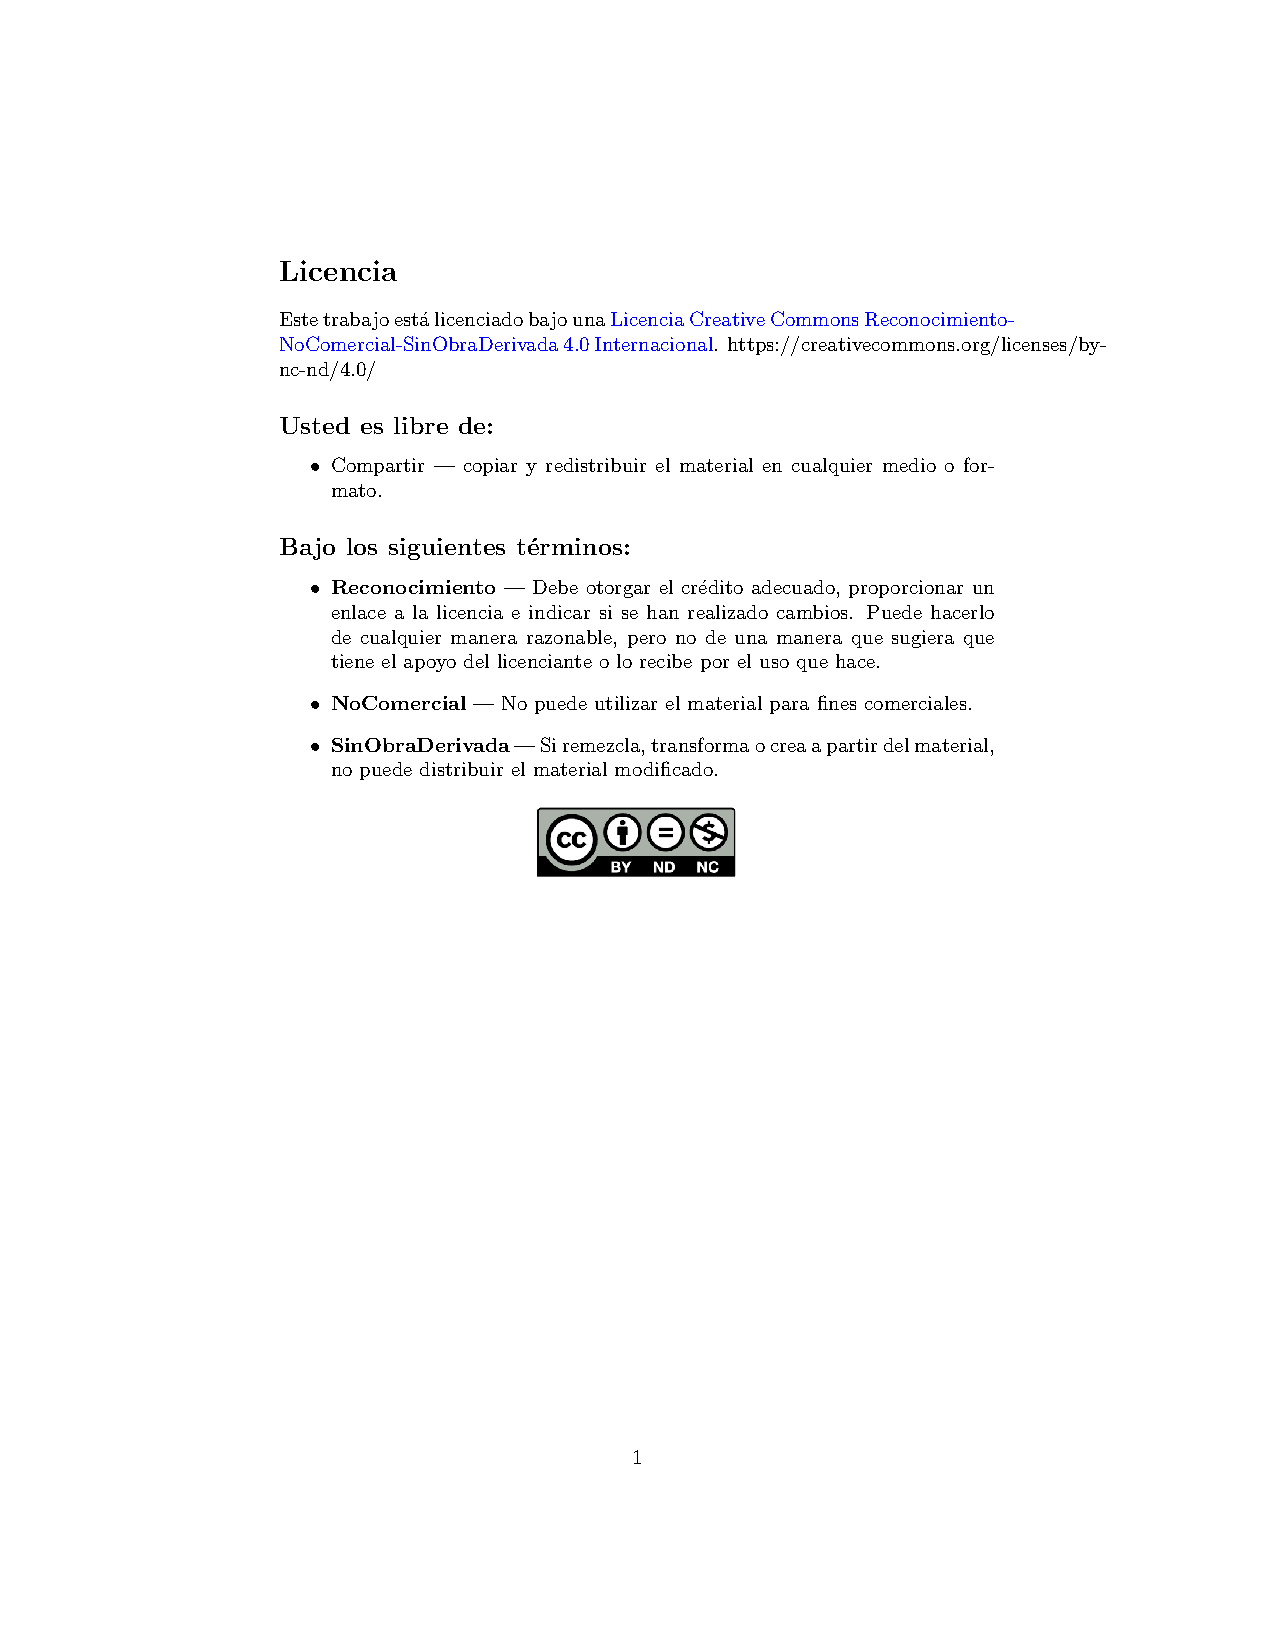
\includepdf[pages=-]{../../../../licencia.pdf}

% Tabla de contenidos

\tableofcontents
\newpage

\chapter{Activos Financieros}

\section{Ejercicio Propuestos}
\subsection*{\textcolor{blue}{Ejercicio Propuesto 1}}


La empresa BARCA, S.A. adquiere un bono el 01/04/20X3 con la intención de negociar los flujos de caja contractuales hasta abril de 20X6, fecha de amortización del bono. Las características del mismo son las siguientes:
\begin{itemize}
    \item Valor de emisión: 98.000 €.
    \item Comisión de adquisición: 2.000 €.
    \item Valor de reembolso: 104.000 €.
    \item Tipo de interés efectivo anual de interés sobre el valor nominal (VN = 100.000 €).
\end{itemize}

Su cuadro de amortización a interés efectivo (7,006\%) es el siguiente:
\begin{table}
\centering
\begin{tabular}{|p{2cm}|p{2cm}|p{2cm}|p{2cm}|p{2cm}|p{2cm}}
    \hline
    Plazo & Intereses devengados & I. Explícitos y reembolso & I. implícitos & Coste amortizado \\
    \hline
    01/04/20X3 & & & & 100.000,00 \\
    \hline
    01/04/20X4 & 6.865,88 & 5.000 & -1.865,88 & 99.865,88 \\
    \hline
    01/04/20X5 & 6.998,65 & 5.000 & -1.998,65 & 99.865,88 \\
    \hline
    01/04/20X6 & 7.136,48 & 109.000 & -2.136,48 & 0,00 \\
    \hline
    \end{tabular}
\end{table}


SE PIDE: Realizar los asientos contables en el libro diario de la sociedad BARCA S.A. relativos a las siguientes operaciones:

\begin{enumerate}[label=\alph*)] % Configura la numeración con "a)"
    \item Contabilización, el 01/04/20X3 de la compra del bono.
    \item A 31/12/20X3, si procede, contabilice el devengo de intereses de la operación del bono.
    \item A 01/04/20X4, contabilice el devengo de intereses de la operación del bono desde enero de 20X4.
    \item A 01/04/20X4, contabilice el cobro de los intereses de la operación del bono.
    \item A 31/12/20X4, si procede, contabilice el devengo de intereses de la operación del bono.
    \item A 01/04/20X5, contabilice el devengo de intereses de la operación del bono.
    \item A 01/04/20X6, contabilice el cobro del reembolso del bono.
\end{enumerate}


\begin{table}[H]
    \centering
    \begin{tabular}{|p{3cm}|p{6cm}|p{3cm}|}
    \hline
    \rowcolor{blue!30}
    \textbf{DEBE} & \textbf{Contabilización 01/04/2023 de la compra de bono} & \textbf{HABER} \\
    \hline
    98000& \cuenta{251} & \\
    \hline
    &  \cuenta{572}& 98000\\
    \hline
    \end{tabular}
\end{table}

\begin{table}[H]
    \centering
    \begin{tabular}{|p{3cm}|p{6cm}|p{3cm}|}
    \hline
    \rowcolor{blue!30}
    \textbf{DEBE} & \textbf{ A 31/12/2023, si procede, contabilice el devengo de los intereses} & \textbf{HABER}\\
    \hline
    3727,03& \cuenta{546} & \\
    \hline
    1378,55&  \cuenta{251}& \\
    \hline
    &  \cuenta{761}& 5105,58 = $98000 \times (1,07006)^{\frac{9}{12}} - 98000$\\
    \hline
    \end{tabular}
\end{table}

\begin{table}[H]
    \centering
    \begin{tabular}{|p{3cm}|p{6cm}|p{3cm}|}
    \hline
    \rowcolor{blue!30}
    \textbf{DEBE} & \textbf{01/04/2024 devengo de los intereses desde Enero 2020} & \textbf{HABER} \\
    \hline
    1272,96 $\rightarrow I=[(100000+3727,03)\times(1,05)^{\frac{3}{12}} - (100000+3727,03)]$& \cuenta{546} & \\
    \hline
    1272,96&  \cuenta{251}& \\
    \hline
    487,47& \cuenta{761} & 1760,23 $\rightarrow I = [(98000+5105,58)\times(1,07006)^{\frac{3}{12}}-(98000+5105,58)]$\\
    \hline
    \end{tabular}
\end{table}

\begin{table}[H]
    \centering
    \begin{tabular}{|p{3cm}|p{6cm}|p{3cm}|}
    \hline
    \rowcolor{blue!30}
    \textbf{DEBE} & \textbf{01/04/2024 cobro intereses de la operación del bono} & \textbf{HABER} \\
    \hline
    5000&  \cuenta{572}& \\
    \hline
    &  \cuenta{546}& 5000\\
    \hline
    \end{tabular}
\end{table}

\begin{table}[H]
    \centering
    \begin{tabular}{|p{3cm}|p{6cm}|p{3cm}|}
    \hline
    \rowcolor{blue!30}
    \textbf{DEBE} & \textbf{31/12/2024 devengo de intereses} & \textbf{HABER} \\
    \hline
    3723,03& \cuenta{546} & \\
    \hline
    1475,76&  \cuenta{251}& \\
    \hline
    & \cuenta{761} & 5202,79 $\rightarrow I = [(99865,88 \times 1,07006)^{\frac{9}{12}} - 99865,88]$\\
    \hline
    \end{tabular}
\end{table}

\begin{table}[H]
    \centering
    \begin{tabular}{|p{3cm}|p{6cm}|p{3cm}|}
    \hline
    \rowcolor{blue!30}
    \textbf{DEBE} & \textbf{04/04/26} & \textbf{HABER} \\
    \hline
    104000&  \cuenta{572}& \\
    \hline
    & \cuenta{541} & 104000\\
    \hline
    \end{tabular}
\end{table}



\newpage
\subsection*{\textcolor{blue}{Ejercicio Propuesto 2}}
En el balance de situación de la empresa “TRAG, S.A.”, a 31 de diciembre del año 2018 figura una letra del tesoro, adquirida el 1 de julio de dicho año, por la que se pagaron 130.000 euros. Su vencimiento es el 30 de junio del año 2020. El nominal de la letra es de 150.000 euros. Se espera que mantener hasta vencimiento este instrumento. El tipo de interés efectivo anual por vencido es del 7,417231\%. La tabla que recoge el coste amortizado a este tipo de interés es la siguiente:

\begin{table}[H]
\centering
\begin{tabular}{|p{2cm}|p{2cm}|p{2cm}|p{2cm}|p{2cm}|p{2cm}|}
    \hline
    Fecha & Pago & Cobros & Intereses devengados (Gastos financieros) & Saldo amortizado & Saldo pendiente de amortizar (Balance) \\
    \hline
    01/07/2018 & 130.000 & 0 & 0 & 0 & 130.000 \\
    \hline
    31/12/2018 & 0 & 0 & 4.734.97 & -4.734.97 & 134.734.97 \\
    \hline
    31/12/2019 & 0 & 0 & 9.993.60 & -9.993.60 & 144.728.57 \\
    \hline
    01/07/2020 & 150.000 & 0 & 5.271.43 & 144.728.57 & 0 \\
    \hline
    \end{tabular}
\end{table}


\textbf{SE PIDE:} Realice las anotaciones contables relacionadas con el enunciado anterior.


\begin{table}[H]
    \centering
    \begin{tabular}{|p{3cm}|p{6cm}|p{3cm}|}
    \hline
    \rowcolor{blue!30}
    \textbf{DEBE} & \textbf{Contabilización el 01/07/2018 de la compra de la letra del tesoro} & \textbf{HABER} \\
    \hline
    130000& \cuenta{251} & \\
    \hline
    &  \cuenta{572}& 130000\\
    \hline
    \end{tabular}
\end{table}

\begin{table}[H]
    \centering
    \begin{tabular}{|p{3cm}|p{6cm}|p{3cm}|}
    \hline
    \rowcolor{blue!30}
    \textbf{DEBE} & \textbf{A 31/12/2018, si procede, contabilice el devengo de intereses} & \textbf{HABER} \\
    \hline
    4734,97&  \cuenta{251}& \\
    \hline
    &  \cuenta{761}& 4734,97\\
    \hline
    \end{tabular}
\end{table}

\begin{table}[H]
    \centering
    \begin{tabular}{|p{3cm}|p{6cm}|p{3cm}|}
    \hline
    \rowcolor{blue!30}
    \textbf{DEBE} & \textbf{A 31/12/2018, si procede, contabilice el cobro de intereses} & \textbf{HABER} \\
    \hline
    &  NPC& \\
    \hline
    \end{tabular}
\end{table}

\begin{table}[H]
    \centering
    \begin{tabular}{|p{3cm}|p{6cm}|p{3cm}|}
    \hline
    \rowcolor{blue!30}
    \textbf{DEBE} & \textbf{A 31/12/2019, si procede, contabilice el devengo de los intereses} & \textbf{HABER} \\
    \hline
    9993,60&  \cuenta{251}& \\
    \hline
    &  \cuenta{761}& 9993,60\\
    \hline
    \end{tabular}
\end{table}


\newpage    
\subsection*{\textcolor{blue}{Ejercicio Propuesto 3}}

La sociedad BENGALS adquiere, el 02/03/2022, 5.000 acciones de la sociedad COWBOYS por importe de 25 €/acción. La operación conlleva unos gastos de gestión que ascienden al 1\% del total de la operación. La inversión se realiza con un carácter de permanencia.

A cierre del ejercicio 2022, estos títulos cotizan a 30 € cada uno, y a cierre del ejercicio 2023 su cotización es de 28 €/acción.

Por necesidades de liquidez, el 23/05/2024 se venden la totalidad de las acciones por un importe de 32 €/acción, con unos costes de transacción del 2\% sobre el precio de venta.

\textbf{SE PIDE:} Contabilizar en el libro diario de BENGALS, S.A. las siguientes operaciones, sin tener en cuenta el posible efecto impositivo:

a) Compra de los títulos a 02/03/2022.

b) Si procede, operaciones derivadas de la valoración de los títulos a 31/12/2022.

c) Si procede, operaciones derivadas de la valoración de los títulos a 31/12/2023.

d) Todas las operaciones derivadas de la venta de los títulos a 23/05/2024.


\begin{table}[H]
    \centering
    \begin{tabular}{|p{3cm}|p{6cm}|p{3cm}|}
    \hline
    \rowcolor{blue!30}
    \textbf{DEBE} & \textbf{Compra de los títulos 02/03/2022} & \textbf{HABER} \\
    \hline
    126250&\cuenta{250}  & \\
    \hline
    &  \cuenta{572}& 126250 = $(5000 \times 25)(1+0,01)$ \\
    \hline
    \end{tabular}
\end{table}

\begin{table}[H]
    \centering
    \begin{tabular}{|p{3cm}|p{6cm}|p{3cm}|}
    \hline
    \rowcolor{blue!30}
    \textbf{DEBE} & \textbf{Si procede, operaciones derivadas de la valoración de los títulos a 31/12/2022} & \textbf{HABER} \\
    \hline
    23750 = $5000 \times 30 = 150000 - 126250$&  \cuenta{250}& \\
    \hline
    &  \cuenta{900} &23750 \\
    \hline
    23750& \cuenta{900} & \\
    \hline
    & \cuenta{133} & 23750\\
    \hline
    \end{tabular}
\end{table}

\begin{table}[H]
    \centering
    \begin{tabular}{|p{3cm}|p{6cm}|p{3cm}|}
    \hline
    \rowcolor{blue!30}
    \textbf{DEBE} & \textbf{Si procede, operaciones derivadas de la valoración de los títulos a 31/12/2023} & \textbf{HABER} \\
    \hline
    10000 &  \cuenta{800}& \\
    \hline
    &  \cuenta{250}& 10000 = $5000 \times 28 = 140000-150000=10000$\\
    \hline
    10000&  \cuenta{133}& \\
    \hline
    &  \cuenta{800}& 10000\\
    \hline
    \end{tabular}
\end{table}

\begin{table}[H]
    \centering
    \begin{tabular}{|p{3cm}|p{6cm}|p{3cm}|}
    \hline
    \rowcolor{blue!30}
    \textbf{DEBE} & \textbf{Todas las operaciones derivadas de la venta de los títulos a 23/05/2024} & \textbf{HABER} \\
    \hline
    156800 = $5000 \times 32 = 160000 - 2 \% \times 160000$&  \cuenta{572}& \\
    \hline
    &  \cuenta{250}& 140000 \\
    \hline
    &  \cuenta{766}& 16800\\
    \hline
    13750 = $23750 - 10000$&  \cuenta{133}& \\
    \hline
    &  \cuenta{802}& 13750\\
    \hline
    13750 &  \cuenta{802}& \\
    \hline
    &  \cuenta{7632}& 13750\\
    \hline
    \end{tabular}
\end{table}

\newpage
\subsection*{\textcolor{blue}{Ejercicio Propuesto 4}}

La empresa EL FIJITIVO, S.L. compra el 01/11/X1, 8.000 acciones del banco MALO, S.A., que cotizan en bolsa a 15 €/acción. Los gastos derivados de la adquisición son 100 €. La inversión tiene carácter especulativo. A 31/12/X1, las acciones de MALO, S.A. cotizan a 13 €/acción y los costes de transacción previstos son de 200 €. El 01/03/X2 se venden las acciones a 12 €/acción con unos gastos de 150 €.

\textbf{SE PIDE:} Contabilice exclusivamente la compra y la venta de las acciones.

\textit{Nos da la pista de que son de carácter especulativo, por lo que debemos de introducir los cambios en la cuenta de Pérdidas y Ganacias}

\begin{table}[H]
    \centering
    \begin{tabular}{|p{3cm}|p{6cm}|p{3cm}|}
    \hline
    \rowcolor{blue!30}
    \textbf{DEBE} & \textbf{Contabilización de la compra de las acciones el 01/11/X1} & \textbf{HABER} \\
    \hline
      120.000 = $8000 \times 15$ &\cuenta{540}  & \\
    \hline
      100 & \cuenta{669} & \\
    \hline
    &  \cuenta{572}& 120.100\\
    \hline
    \end{tabular}
\end{table}


\subsubsection*{Anotaciones extra:}
\begin{itemize}
    \item Los gastos son de 100 €.
    \item El VR = $8000 \times 12 = 96000$ (no se tiene en cuenta cuanto cuesta venderlos).
    \item El VC = $8000 \times 15 = 120000$
    \item El VR = $8000 \times 13 = 104000 \rightarrow$ debemos de contabilizar una pérdida de 16000 = $120000 - 104000$, para anotarlo debemos de usar la cuenta del grupo 6 (Pérdidas de la cartera de la negociación). \textit{Lo recogemos directamente, por ende no debemos de dotar de deterioro previamente.}
\end{itemize}

\begin{table}[H]
    \centering
    \begin{tabular}{|p{3cm}|p{6cm}|p{3cm}|}
    \hline
    \rowcolor{blue!30}
    \textbf{DEBE} & \textbf{Contabilización, el 01/03/X2 de la venta de las acciones} & \textbf{HABER} \\
    \hline
    95.850 = $(8000 \times 12) - 150 $&  \cuenta{572}& \\
    \hline
    8150 &  \cuenta{666}& \\
    \hline
    &  \cuenta{540}& 104.000\\
    \hline
    \end{tabular}
\end{table}

Si suponemos el caso en el que el importe de la venta es de 6000 €, debemos de realizar el cociente $\frac{104000}{8000} = 13$ \euro/acción, por lo que tendríamos $6000 \times 13 = 78000$, de manera que si el importe neto es 71.850, debemos de contabilizar una pérdida de 6150.

\newpage
\section{Otros Ejercicios}


\subsection*{\textcolor{red}{\textbf{Ejercicio 1}}}

El banco EUROPA, S.A. concede un préstamo a la empresa COPA, S.A. por un valor nominal de 50.000 € el día 1 de marzo de 2019 con un vencimiento a tres años y un valor de reembolso de 52.000 €, al tipo de interés nominal del 5\%. Los gastos de la operación (que corren a cargo de la empresa COPA) ascienden a 1.000 €. El tipo de interés efectivo de la operación es del 6,2535\%. El cuadro de amortización calculado en base al tipo de interés efectivo es el siguiente:

\begin{table}[H]
\centering
\begin{tabular}{|c|c|c|c|p{4cm}|}
    \hline
    Plazo & Intereses Devengados & Pagos & Saldo amortizado & Saldo pendiente de amortizar \\
    \hline
    01/01/2019 & & & & 50.000 \\
    \hline
    31/12/2019 & 3.126,75 & 2.500 & 626,75 & 50.626,75 \\
    \hline
    31/12/2020 & 3.165,94 & 2.500 & 665,94 & 50.292,69 \\
    \hline
    31/12/2021 & 3.207,58 & 54.500 & 51.292,69 & 0 \\
    \hline
\end{tabular}
\end{table}

\textbf{SE PIDE:} Contabilizar las siguientes operaciones:

\begin{enumerate}[label=\alph*)]
    \item Concesión del crédito a 01/01/2019.
    
    \begin{table}[H]
        \centering
        \begin{tabular}{|p{3cm}|p{6cm}|p{3cm}|}
        \hline
        \rowcolor{blue!30}
        \textbf{DEBE} & \textbf{Concesión del crédito a 01/01/2019} & \textbf{HABER} \\
        \hline
        50.000 & (252) Créditos a largo plazo & \\
        \hline
        & (572) Bancos c/c & 50.000 \\
        \hline
        \end{tabular}
        \caption{Asiento a. Ejercicio 1.}
        \label{tabla:asiento1ej1T2}
    \end{table}

    \item Contabilización de las operaciones necesarias a 31/12/2019.
    
    \begin{table}[H]
        \centering
        \begin{tabular}{|p{3cm}|p{6cm}|p{3cm}|}
        \hline
        \rowcolor{blue!30}
        \textbf{DEBE} & \textbf{Contabilización de las operaciones necesarias a 31/12/2019} & \textbf{HABER} \\
        \hline
        2.500 & (572) Bancos c/c & \\
        \hline
        626,75 & (252) Créditos a largo plazo & \\
        \hline
        & (762) Ingresos de créditos & 3.126,75 \\
        \hline
        \end{tabular}
        \caption{Asiento b. Ejercicio 1.}
        \label{tabla:asiento2ej1T2}
    \end{table}


    \item Contabilización de la reclasificación del derecho de cobro a 31/12/2020.
    \begin{table}[H]
        \centering
        \begin{tabular}{|p{3cm}|p{6cm}|p{3cm}|}
        \hline
        \rowcolor{blue!30}
        \textbf{DEBE} & \textbf{Devengo de intereses a 31/12/2020} & \textbf{HABER} \\
        \hline
        2.500 & (572) Bancos c/c & \\
        \hline
        665,94 & (252) Créditos a largo plazo & \\
        \hline
        & (762) Ingresos de créditos & 3.165,94 \\
        \hline
        \end{tabular}
        \caption{Asiento c-1. Ejercicio 1.}
        \label{tabla:asiento3ej1T2}
    \end{table}
    \begin{align*}
        \text{Saldo de la cuenta (252) Créditos a largo plazo} = \\ = 50.000 + 626,75 + 665,94 = 51.292,69 \text{ \euro}
    \end{align*}

    \begin{table}[H]
        \centering
        \begin{tabular}{|p{3cm}|p{6cm}|p{3cm}|}
        \hline
        \rowcolor{blue!30}
        \textbf{DEBE} & \textbf{Contabilización de la reclasificación del derecho de cobro a 31/12/2020} & \textbf{HABER} \\
        \hline
        51.292,69 & (542) Créditos a corto plazo & \\
        \hline
        & (252) Créditos a largo plazo & 51.292,69 \\
        \hline
        \end{tabular}
        \caption{Asiento c-2. Ejercicio 1.}
        \label{tabla:asiento4ej1T2}
    \end{table}

    \item Contabilización de la cancelación del derecho de cobro EXCLUSIVAMENTE por su valor de reembolso el 31/12/2021.
    
    \begin{table}[H]
        \centering
        \begin{tabular}{|p{3cm}|p{6cm}|p{3cm}|}
        \hline
        \rowcolor{blue!30}
        \textbf{DEBE} & \textbf{Devengo de intereses a 31/12/2021} & \textbf{HABER} \\
        \hline
        2.500 & (572) Bancos c/c & \\
        \hline
        707,58 & (542) Créditos a largo plazo & \\
        \hline
        & (762) Ingresos de créditos & 3.207,58 \\
        \hline
        \end{tabular}
        \caption{Asiento d-1. Ejercicio 1.}
        \label{tabla:asiento5ej1T2}
    \end{table}
    \begin{align*}
        \text{Saldo de la cuenta (542) Créditos a corto plazo} = \\ = 51.292,69 + 707,58 \approx \text{52.000} \text{ \euro}
    \end{align*}

    \begin{table}[H]
        \centering
        \begin{tabular}{|p{3cm}|p{6cm}|p{3cm}|}
        \hline
        \rowcolor{blue!30}
        \textbf{DEBE} & \textbf{Contabilización de la cancelación del derecho de cobro EXCLUSIVAMENTE por su valor de reembolso el 31/12/2021} & \textbf{HABER} \\
        \hline
        52.000 & (572) Bancos c/c & \\
        \hline
        & (542) Créditos a corto plazo & 52.000 \\
        \hline
        \end{tabular}
        \caption{Asiento d-2. Ejercicio 1.}
        \label{tabla:asiento6ej1T2}
    \end{table}
\end{enumerate}

\newpage 
\subsection*{\textcolor{red}{\textbf{Ejercicio 2}}}
La empresa TUNA, S.A. concede el 1 de enero de 2018 un crédito de 10.000 € a la empresa VELVAT S.A., a devolver en 3 años en cuotas constantes anuales y cuyo cuadro de amortización según el tipo de interés efectivo al 7\% es el siguiente:

\begin{table}[H]
\centering
\begin{tabular}{|c|c|c|c|c|}
    \hline
    Fecha & Pago & Cobros (cuota) & Intereses & Capital \\
    \hline
    01/01/2018 & 10.000 & & & 10.000 \\
    \hline
    31/12/2018 & 3.810,52 & 700 & 3.110,52 & 6.889,48 \\
    \hline
    31/12/2019 & 3.810,52 & 482,26 & 3.328,25 & 3.561,23 \\
    \hline
    31/12/2020 & 3.810,52 & 249,29 & 3.561,23 & 0,00 \\
    \hline
\end{tabular}
\end{table}

\textbf{SE PIDE:} Contabilice los siguientes apartados para la empresa TUNA, S.A.:

\begin{enumerate}[label=\alph*)]
    \item Asiento contable de la formalización del crédito el 01/01/2018.
    
    \begin{table}[H]
        \centering
        \begin{tabular}{|p{3cm}|p{6cm}|p{3cm}|}
        \hline
        \rowcolor{blue!30}
        \textbf{DEBE} & \textbf{Formalización del crédito el 01/01/2018} & \textbf{HABER} \\
        \hline
        3.110,52 & (542) Créditos a corto plazo & \\
        \hline
        6.889,48 & (252) Créditos a largo plazo & \\
        \hline
        & (572) Bancos c/c & 10.000 \\
        \hline
        \end{tabular}
    \end{table}

    \item Asiento contable del cobro de la primera cuota el 31/12/2018.
    
    \begin{table}[H]
        \centering
        \begin{tabular}{|p{3cm}|p{6cm}|p{3cm}|}
        \hline
        \rowcolor{blue!30}
        \textbf{DEBE} & \textbf{Cobro de la primera cuota el 31/12/2018} & \textbf{HABER} \\
        \hline
        3.810,52 & (572) Bancos c/c & \\
        \hline
        & (542) Créditos a corto plazo & 3.110,52 \\
        \hline
        & (762) Ingresos de créditos & 700 \\
        \hline
        \end{tabular}
    \end{table}
    \item Asiento contable de la reclasificación del derecho de cobro el 31/12/2019.
    \begin{table}[H]
        \centering
        \begin{tabular}{|p{3cm}|p{6cm}|p{3cm}|}
        \hline
        \rowcolor{blue!30}
        \textbf{DEBE} & \textbf{Reclasificación del derecho de cobro el 31/12/2019} & \textbf{HABER} \\
        \hline
        3.561,23 & (542) Créditos a corto plazo & \\
        \hline
        & (252) Créditos a largo plazo & 3.561,23 \\
        \hline
        \end{tabular}
    \end{table}
    \item Asiento contable del cobro de la última cuota el 31/12/2020.
    \begin{table}[H]
        \centering
        \begin{tabular}{|p{3cm}|p{6cm}|p{3cm}|}
        \hline
        \rowcolor{blue!30}
        \textbf{DEBE} & \textbf{Cobro de la última cuota el 31/12/2020} & \textbf{HABER} \\
        \hline
        3.810,52 & (572) Bancos c/c & \\
        \hline
        & (542) Créditos a corto plazo & 3.561,23 \\
        \hline
        & (762) Ingresos de créditos & 249,29 \\
        \hline
        \end{tabular}
    \end{table}
\end{enumerate}

\newpage
\subsection*{\textcolor{red}{\textbf{Ejercicio 3}}}

La sociedad PANDEMIA, S.A. adquiere a 1 de junio de 2020 tres partidas de instrumentos financieros con las siguientes características (todas las operaciones se realizan a través de transferencia bancaria):

- 300 acciones de la sociedad OMS, S.A. adquisición que se realiza de forma puntual con el objetivo de mantenerlas como inversión a l/p sin expectativa de ganancias en el corto plazo. El precio unitario es de 100 € y llevan aparejados unos gastos de adquisición del 2\% sobre el precio total.

- 300 acciones de la sociedad GLOBAL, S.A. que adquiere con fines especulativos. El precio unitario es de 150 € y llevan aparejados unos gastos del 2\% sobre el precio total.

- 300 obligaciones de la sociedad MUNDIAL, S.A. que incluye en la categoría de activos financieros a valor razonable con cambios en el patrimonio neto. El precio unitario es de 200 € y llevan aparejados unos gastos del 2\% sobre el precio total.

Las tres sociedades cotizan en bolsa por lo que a 31 de diciembre de 2020 el valor de los títulos asciende a: OMS: 125 €; GLOBAL: 200 € y MUNDIAL: 180 €.

Por necesidades de liquidez vende todos los instrumentos financieros el 1 de febrero de 2021 a un precio unitario igual para todas de 150 €.

\begin{enumerate}[label=\alph*)]
    \item A 1/06/2020, contabilización de la adquisición de las acciones de OMS, S.A.
    \begin{align*}
        PA = \\ 
        = (300 \text{acciones} \times 100 \text{\euro/acción}) \times 1,02 = 30.600 \text{\euro}
    \end{align*}
    \begin{table}[H]
        \centering
        \begin{tabular}{|p{3cm}|p{6cm}|p{3cm}|}
        \hline
        \rowcolor{blue!30}
        \textbf{DEBE} & \textbf{A 01/06/2020, contabilización de la adquisición de las acciones de OMS, S.A.} & \textbf{HABER} \\
        \hline
        30.600 & (250) Inversiones financieras a largo plazo en instrumentos de patrimonio & \\
        \hline
        & (572) Bancos c/c & 30.600 \\
        \hline
        \end{tabular}
    \end{table}
    \item A 1/06/2020, contabilización de la adquisición de las acciones de GLOBAL, S.A.
    
    \begin{align*}
        PA = \\ 
        = (300 \text{acciones} \times 150 \text{\euro/acción}) \times 1,02 = 45.900 \text{\euro}
    \end{align*}

    \begin{table}[H]
        \centering
        \begin{tabular}{|p{3cm}|p{6cm}|p{3cm}|}
        \hline
        \rowcolor{blue!30}
        \textbf{DEBE} & \textbf{A 01/06/2020, contabilización de la adquisición de las acciones de GLOBAL, S.A.} & \textbf{HABER} \\
        \hline
        45.000 & (540) Inversiones financieras a corto plazo en instrumentos de patrimonio & \\
        \hline
        900 & (669) Otros gastos financieros & \\
        \hline
        & (572) Bancos c/c & 45.900 \\
        \hline
        \end{tabular}
    \end{table}

    \item A 1/06/2020, contabilización de la adquisición de las obligaciones de MUNDIAL, S.A.
    
    \begin{align*}
        PA = \\ 
        = (300 \text{obligaciones} \times 200 \text{\euro/obligación}) \times 1,02 = 61.200 \text{\euro}
    \end{align*}
    \begin{table}[H]
        \centering
        \begin{tabular}{|p{3cm}|p{6cm}|p{3cm}|}
        \hline
        \rowcolor{blue!30}
        \textbf{DEBE} & \textbf{A 01/06/2020, contabilización de la adquisición de las obligaciones de MUNDIAL, S.A.} & \textbf{HABER} \\
        \hline
        61.200 & (541) Valores representativos de deuda a corto plazo & \\
        \hline
        & (572) Bancos c/c & 61.200 \\
        \hline
        \end{tabular}
    \end{table}
    \item A 31/12/2020, contabilización de las operaciones relativas a las acciones de OMS, S.A.
    
    \begin{align*}
        VR = \\ 
        = 300 \text{acciones} \times 125 \text{\euro/acción} = 37.500 \text{\euro}
    \end{align*}
    \begin{align*}
        Beneficio = \\ 
        = 37.500 - 30.600 = 6.900 \text{\euro}
    \end{align*}

    \begin{table}[H]
        \centering
        \begin{tabular}{|p{3cm}|p{6cm}|p{3cm}|}
        \hline
        \rowcolor{blue!30}
        \textbf{DEBE} & \textbf{A 31/12/2020, contabilización de las operaciones relativas a las acciones de OMS, S.A.} & \textbf{HABER} \\
        \hline
        6.900 & (250) Inversiones financieras a largo plazo en instrumentos de patrimonio & \\
        \hline
        & (900) Beneficios de activos financieros a valor razonable con cambios en el patrimonio neto & 6.900 \\
        \hline
        6.900 & (900) Beneficios de activos financieros a valor razonable con cambios en el patrimonio neto & \\
        \hline
        & (133) Ajustes en la valoración de activos financieros con cambios en el patrimonio neto & 6.900 \\
        \hline
        \end{tabular}
    \end{table}

    \item A 31/12/2020, contabilización de las operaciones relativas a las acciones de GLOBAL, S.A.
    
    \begin{align*}
        VR = \\ 
        = 300 \text{acciones} \times 200 \text{\euro/acción} = 60.000 \text{\euro}
    \end{align*}
    \begin{align*}
        Beneficio =  \\ 
        = 300 \times (200-150) = \text{15.000} \text{\euro}
    \end{align*}

    \begin{table}[H]
        \centering
        \begin{tabular}{|p{3cm}|p{6cm}|p{3cm}|}
        \hline
        \rowcolor{blue!30}
        \textbf{DEBE} & \textbf{A 31/12/2020, contabilización de las operaciones relativas a las acciones de GLOBAL, S.A.} & \textbf{HABER} \\
        \hline
        15.000 & (540) Inversiones financieras a corto plazo en instrumentos de patrimonio & \\
        \hline
        & (7630) Beneficios cartera de negociación & 15.000 \\
        \hline
        \end{tabular}
    \end{table}

    \item A 31/12/2020, contabilización de las operaciones relativas a las obligaciones de MUNDIAL, S.A.
    
    \begin{align*}
        \text{Precio adquisición} = \text{61.200} \text{\euro} \\ \text{A 31 de diciembre } \rightarrow \text{cotización} = 180 \text{\euro/obligación} \\  \Rightarrow \text{61.200}  (300 \times 180) = 7.200 \text{\euro}
    \end{align*}

    \begin{table}[H]
        \centering
        \begin{tabular}{|p{3cm}|p{6cm}|p{3cm}|}
        \hline
        \rowcolor{blue!30}
        \textbf{DEBE} & \textbf{A 31/12/2020, contabilización de las operaciones relativas a las obligaciones de MUNDIAL, S.A.} & \textbf{HABER} \\
        \hline
        7.200 & (800) Pérdidas de activos financieros a valor razonable con cambios en el patrimonio neto & \\
        \hline
        & (541) Valores representativos de deuda a corto plazo & 7.200 \\
        \hline
        7.200 & (133) Ajustes en la valoración de activos financieros con cambios en el patrimonio neto & \\
        \hline
        & (800) Pérdidas de activos financieros a valor razonable con cambios en el patrimonio neto & 7.200 \\
        \hline
        \end{tabular}
    \end{table}

    \item A 01/02/2021, contabilización, exclusivamente, de la venta de las acciones de OMS, S.A.
    
    \begin{align*}
        \text{Se venden} \rightarrow 300 \times 150 = 45.000 \text{\euro}
    \end{align*}

    Debemos de mirar el saldo de la cuenta (250) en el libro mayor:

    \begin{figure}[H]
        \centering
        \begin{tikzpicture}
            \draw (0,0) -- (5,0);
            \node at (2.5,0.3) {(250) IF l/p I.P.};
            \draw (2.6,0) -- (2.6,-2.7);
            \node[anchor=west] at (0.1,-0.5) {30.600 (D)};
            \node[anchor=west] at (0.1,-1.5) {6.900 (D)};
            \node[anchor=west] at (0.1,-2.5) {SD = 37.500};
        \end{tikzpicture}
        \caption{Contabilización de la venta de las acciones de OMS, S.A.}
    \end{figure}

    \begin{table}[H]
        \centering
        \begin{tabular}{|p{3cm}|p{6cm}|p{3cm}|}
        \hline
        \rowcolor{blue!30}
        \textbf{DEBE} & \textbf{A 01/02/2021, contabilización, exclusivamente, de la venta de las acciones de OMS, S.A.} & \textbf{HABER} \\
        \hline
        45.000 & (572) Bancos c/c & \\
        \hline
        & (250) Inversiones financieras a largo plazo en instrumentos de patrimonio & 37.500 \\
        \hline
        & (766) Beneficios en participaciones y VRD & 7.500 \\
        \hline
        \end{tabular}
    \end{table}

    Hasta aquí estaría completo el ejercicio, pero debemos de regularizar la cuenta de patrimonio vinculada a esta inversión.

    \begin{table}[H]
        \centering
        \begin{tabular}{|p{3cm}|p{6cm}|p{3cm}|}
        \hline
        \rowcolor{blue!30}
        \textbf{DEBE} & \textbf{Regularización del patrimonio neto} & \textbf{HABER} \\
        \hline
        6.900 & (133) Ajustes en la valoración de AF (PN) & \\
        \hline
        & (802) Transferencia de beneficios de AF (PN) & 6.900 \\
        \hline
        6.900 & (802) Transferencia de beneficios de AF (PN) & \\
        \hline
        & (7632) Beneficios de activos financieros a valor razonable con cambios en el patrimonio neto & 6.900 \\
        \hline
        \end{tabular}
    \end{table}

    \item A 01/02/2021, contabilización de la venta de las acciones de GLOBAL, S.A.
    
    \begin{align*}
        \text{A 31 de diciembre estas acciones estaban valoradas a 200 \euro/acción} \\
        \text{Se vende } \rightarrow 150 \text{ \euro/acción} \\
        \Rightarrow \text{Pérdida}
    \end{align*}

    \begin{table}[H]
        \centering
        \begin{tabular}{|p{3cm}|p{6cm}|p{3cm}|}
        \hline
        \rowcolor{blue!30}
        \textbf{DEBE} & \textbf{A 01/02/2021, contabilización de la venta de las acciones de GLOBAL, S.A.} & \textbf{HABER} \\
        \hline
        45.000 & (572) Bancos c/c & \\
        \hline
        15.000 & (666) Beneficios en participaciones y valores representativos de deuda & \\
        \hline
        & (540) Inversiones financieras a corto plazo en instrumentos de patrimonio & 60.000 \\
        \hline
        \end{tabular}
    \end{table}



    \item A 01/02/2021, contabilización, exclusivamente, de la venta de las obligaciones de MUNDIAL, S.A.
    
    \begin{align*}
        \text{Saldo} = \text{61.200} - \text{7.200} = \text{54.000} \text{\euro} \\
        \text{Se venden} \text{ 300 Obligaciones} \times 150 \text{\euro/obligación} = \text{45.000} \text{\euro}
    \end{align*}

    \begin{table}[H]
        \centering
        \begin{tabular}{|p{3cm}|p{6cm}|p{3cm}|}
        \hline
        \rowcolor{blue!30}
        \textbf{DEBE} & \textbf{A 01/02/2021, contabilización, exclusivamente, de la venta de las obligaciones de MUNDIAL, S.A.} & \textbf{HABER} \\
        \hline
        45.000 & (572) Bancos c/c & \\
        \hline
        9.000 & (6668) Pérdidas VRD c/p & \\
        \hline
        & (541) Valores representativos de deuda a corto plazo & 54.000 \\
        \hline
        \end{tabular}
    \end{table}

    También se tendría que regularizar la cuenta de patrimonio neto vinculada a esta inversión.

    \begin{table}[H]
        \centering
        \begin{tabular}{|p{3cm}|p{6cm}|p{3cm}|}
        \hline
        \rowcolor{blue!30}
        \textbf{DEBE} & \textbf{Regularización del patrimonio neto} & \textbf{HABER} \\
        \hline
        7.200 & (902) Transferencia de pérdidas AF (PN) & \\
        \hline
        & (133) Ajustes en la valoración de AF (PN) & 7.200 \\
        \hline
        7.200 & (6632) Pérdidas de activos financieros a valor razonable con cambios en el patrimonio neto & \\
        \hline
        & (902) Transferencia de pérdidas AF (PN) & 7.200 \\
        \hline
        \end{tabular}
    \end{table}
\end{enumerate}

\newpage 
\subsection*{\textcolor{red}{\textbf{Ejercicio 4}}}


La empresa MOU adquiere el 01/01/2020 un paquete de 200 obligaciones emitidas por FLO en esa misma fecha y amortizables el 31/12/2021 y que cotizan en mercado secundario. Los títulos tienen un valor nominal de 1.000 € y un valor de reembolso de 1.100 € cada uno. En las condiciones de emisión se estableció un tipo de interés nominal del 5\%, pagadero el último día del ejercicio. La empresa MOU pagó 212.000 € por los títulos, y comisiones por 500 €. MOU tiene la intención de mantenerlos hasta el vencimiento. El cuadro de amortización de las obligaciones se muestra en la siguiente tabla calculado con un tipo de interés efectivo del 6,416\%:

\begin{table}[H]
\centering
\begin{tabular}{|p{2cm}|p{2cm}|p{2cm}|p{2cm}|p{2cm}|p{2cm}|}
    \hline
    Fecha & Pago & Cobros & Intereses devengados (Ingresos financieros) & Saldo amortizado & Saldo pendiente de amortizar (Balance) \\
    \hline
    01/01/2020 & 212.500 & & & & 212.500 \\
    \hline
    31/12/2020 & 10.000 & & 13.633 & 3.633 & 216.133 \\
    \hline
    31/12/2021 & 230.000 & & 13.867 & 216.133 & 0 \\
    \hline
\end{tabular}
\end{table}

\textbf{SE PIDE:} Realizar los asientos contables en el libro diario relativos a las siguientes operaciones:

a) Asiento contable de la adquisición de las obligaciones por MOU.

La empresa tiene la intención de mantener los títulos hasta el vencimiento, por lo que se clasificarán como \textit{activos financieros a coste amortizado}.

Sabemos que inicialmente, los clasificados en esta categoría se valoran inicialmente por su valor razonable.

\begin{table}[H]
    \centering
    \begin{tabular}{|p{3cm}|p{6cm}|p{3cm}|}
    \hline
    \rowcolor{blue!30}
    \textbf{DEBE} & \textbf{Asiento contable adquisición de las obligaciones por MOU} & \textbf{HABER} \\
    \hline
    212.500 & (251) Valores representativos de deuda a largo plazo & \\
    \hline
    & (572) Banco X c/c & 212.500 \\
    \hline
    \end{tabular}
\end{table}


b) Asiento contable reflejo de los intereses a 31/12/2020 realizado por MOU.

Aunque los totales devengados asciendan a 13.633 \euro, solo se cobran los explícitos (10.000 \euro).


\begin{table}[H]
    \centering
    \begin{tabular}{|p{3cm}|p{6cm}|p{3cm}|}
    \hline
    \rowcolor{blue!30}
    \textbf{DEBE} & \textbf{Asiento contable reflejo de los intereses a 31/12/2020 realizado por MOU} & \textbf{HABER} \\
    \hline
    10.000 & (572) Banco X c/c & \\
    \hline
    3.633 & (251) Valores representativos de deuda a largo plazo & \\
    \hline
    & (761) Ingresos valores representativos de deuda & 13.633 \\
    \hline
    \end{tabular}
\end{table}

\textbf{Si el valor razonable de los títulos a 31/12/2020 fuera de 1.050 €/obligación:}

c) Asiento contable reflejo del valor de mercado de las obligaciones a 31/12/2020 realizado por MOU.



\begin{align*}
    \text{Según el cuadro de amortización, el valor de inversión:} & \quad 216.133 \, \text{\euro} \\
    \text{Según el valor razonable:} & \quad 200 \times 1.050 \, \text{\euro/obligación} = 210.000 \, \text{\euro} \\
    \text{Pérdida:} & \quad 216.133 \, \text{\euro} - 210.000 \, \text{\euro} = 6.133 \, \text{\euro}
\end{align*}

\begin{table}[H]
    \centering
    \begin{tabular}{|p{3cm}|p{6cm}|p{3cm}|}
    \hline
    \rowcolor{blue!30}
    \textbf{DEBE} & \textbf{Asiento contable reflejo del valor de mercado de las obligaciones a 31/12/2020 realizado por MOU} & \textbf{HABER} \\
    \hline
    6.133 & (696) Pérdidas por deterioro de participaciones y valores representativos de deuda a largo plazo & \\
    \hline
    & (297) Deterioro de valor de valores representativos de deuda a largo plazo & 6.133 \\
    \hline
    \end{tabular}
\end{table}

Sin tener en cuenta el asiento anterior:

d) Asiento contable reflejo de los intereses y reembolso de los títulos a 31/12/2021 por MOU.

Como finaliza la inversión, la empresa recibe el importe de los títulos y los intereses devengados.

\begin{table}[H]
    \centering
    \begin{tabular}{|p{3cm}|p{6cm}|p{3cm}|}
    \hline
    \rowcolor{blue!30}
    \textbf{DEBE} & \textbf{Asiento contable reflejo de los intereses y reembolso de los títulos a 31/12/2021 por MOU} & \textbf{HABER} \\
    \hline
    230.000 & (572) Banco X c/c & \\
    \hline
    & (541) Valores representativos de deuda a corto plazo & 216.133 \\
    \hline
    & (761) Ingresos VRD & 13.867 \\
    \hline
    \end{tabular}
\end{table}

\newpage
\subsection*{\textcolor{red}{\textbf{Ejercicio 5}}}

La sociedad INVERSORA, S.A. adquiere a 1 de diciembre de 2020 un paquete de 500 acciones de la sociedad cotizada TELEMARKETING a un precio unitario de 120 € la acción. Esta operación lleva unos gastos de adquisición del 2\% sobre el precio total. La política de la empresa con estas acciones es mantenerlas a largo plazo sin un marcado carácter especulativo, optando por no valorarlas a coste. A 31 de diciembre de 2020 estas acciones cotizan a 90 € la acción.

El 1 de marzo de 2021 la empresa decide considerar esa cartera como especulativa y espera venderla en unos días ya que el precio ha subido. El 20 de marzo de 2021 la empresa decide vender la cuarta parte de dichas acciones, siendo la cotización en dicho día de 130 € la acción.

SE PIDE: Contabilizar en la empresa INVERSORA S.A., las siguientes situaciones:

\textbf{a) Asiento relativo a la compra de las acciones de TELEMARKETING a 01/12/2020.}

\begin{align*}
    \text{Precio de adquisición} = 500 \times 120 \times 1,02 = 61.200 \text{ \euro}
\end{align*}

\begin{table}[H]
    \centering
    \begin{tabular}{|p{3cm}|p{6cm}|p{3cm}|}
    \hline
    \rowcolor{blue!30}
    \textbf{DEBE} & \textbf{Asiento relativo a la compra de las acciones de TELEMARKETING a 01/12/2020} & \textbf{HABER} \\
    \hline
    61.200 & (250) Inversiones financieras a largo plazo en instrumentos de patrimonio & \\
    \hline
    & (572) Bancos c/c & 61.200 \\
    \hline
    \end{tabular}
\end{table}





\textbf{b) Asiento/s relativo/s a las acciones de TELEMARKETING a 31/12/2020.
}
\begin{align*}
    \text{Estas a 31/12 cotizan a 90 \euro/acción, por lo que } 500 \times 90 = \text{45.000} \text{ \euro} \\
    \text{Valor contable} = 61.200 \text{ \euro} \\
    \text{Pérdida} = 61.200 - 45.000 = 16.200 \text{ \euro}
\end{align*}

\begin{table}[H]
    \centering
    \begin{tabular}{|p{3cm}|p{6cm}|p{3cm}|}
    \hline
    \rowcolor{blue!30}
    \textbf{DEBE} & \textbf{Asiento/s relativo/s a las acciones de TELEMARKETING a 31/12/2020} & \textbf{HABER} \\
    \hline
    16.200 & (800) Pérdidas en activos financieros a valor razonable con cambios en el patrimonio neto & \\
    \hline
    & (250) Inversiones financieras a largo plazo instrumentos de patrimonio & 16.200 \\
    \hline
    16.200 & (133) Ajustes en valoración de activos financieros a valor razonable con cambios en el patrimonio neto & \\
    \hline
    & (800) Pérdidas en activos financieros a valor razonable con cambios en el patrimonio neto & 16.200 \\
    \hline
    \end{tabular}
\end{table}


\textbf{c) Clasificación, si procede, en la empresa INVERSORA, S.A. de las acciones de TELEMARKETING el 01/03/2021.}

Como se menciona que los adquiere con carácter especulativo, es decir, como un activo financiero a VR con cambios en la cuenta de pérdidas y ganancias ya que espera venderlos en un corto plazo.

\begin{table}[H]
    \centering
    \begin{tabular}{|p{3cm}|p{6cm}|p{3cm}|}
    \hline
    \rowcolor{blue!30}
    \textbf{DEBE} & \textbf{Clasificación, si procede, en la empresa INVERSORA, S.A. de las acciones de TELEMARKETING el 01/03/2021} & \textbf{HABER} \\
    \hline
    16.200 & (902) Transferencia de pérdidas AF a valor razonable con cambios en el patrimonio neto & \\
    \hline
    & (133) Ajustes en valoración de activos financieros con cambios en el patrimonio neto & 16.200 \\
    \hline
    16.200 & (6632) Pérdidas de activos financieros a valor razonable con cambios en el patrimonio neto & \\
    \hline
    & (902) Transferencia de pérdidas AF a valor razonable con cambios en el patrimonio neto & 16.200 \\
    \hline
    \end{tabular}
\end{table}

\textbf{d) Asiento relativo a la venta de los títulos el 20/03/2021.}

\begin{align*}
    \text{La empresa decide vender } \frac{1}{4} \times 500 = 125 \text{ acciones} \\
    \text{Precio de venta} = 125 \times 130 = 16.250 \text{ \euro}\\
    \text{En diciembre cotizaban a 90 \euro/acción} \\
    \text{Damos de baja a } 125 \text{ acciones} \times 90 \text{ \euro/acción} = 11.250 \text{ \euro} \\
    \text{Ganancia} = 16.250 - 11.250 = 5.000 \text{ \euro}
\end{align*}

\begin{table}[H]
    \centering
    \begin{tabular}{|p{3cm}|p{6cm}|p{3cm}|}
    \hline
    \rowcolor{blue!30}
    \textbf{DEBE} & \textbf{Asiento relativo a la venta de los títulos el 20/03/2021} & \textbf{HABER} \\
    \hline
    16.250 & (572) Bancos c/c (125 x 130) & \\
    \hline
    & (540) Inversiones financieras a corto plazo en instrumentos de patrimonio & 11.250 \\
    \hline
    & (766) Beneficios en participaciones y VRD & 5.000 \\
    \hline
    \end{tabular}
\end{table}

\begin{tcolorbox}
    Como en el apartado c) se hizo el ajuste de la cuenta de PN, en este caso no hay que regularizar nada como consecuencia de la venta, puesto que ya estaban reclasificadas como activos financieros a vR con cambios en la cuenta de pérdidas y ganancias.
\end{tcolorbox}

\newpage
\subsection*{\textcolor{red}{\textbf{Ejercicio 6}}}

La empresa TRESA realiza una inversión en bonos, con vencimiento a tres años, en las siguientes condiciones:

A 01/03/X1, adquiere en el mercado 5.000 bonos de 10 € nominales, al 95\%.

Estos títulos devengan un cupón anual postpagable del 1,5\%. Los gastos de la operación anteriores, a cargo de TRESA se estiman en el 1\% sobre el nominal. La empresa espera mantener estas inversiones hasta su vencimiento.

El tipo de interés efectivo de la operación es del 2,9117\%. El cuadro financiero que recoge el coste amortizado de los bonos es el siguiente:

\begin{table}[H]
\centering
\begin{tabular}{|p{2cm}|p{2cm}|p{2cm}|p{2cm}|p{2cm}|}
    \hline
    Fecha & Inter. Devengados TAE & I. Explícitos y reembolso (Cobros) & I. Implícitos & Coste amortizado \\
    \hline
    01/03/20X1 & & & & 48.000 \\
    \hline
    01/03/20X2 & 1.398 & 750 & 648 & 48.648 \\
    \hline
    01/03/20X3 & 1.416 & 750 & 666 & 49.314 \\
    \hline
    01/03/20X4 & 1.436 & 50.750 & 686 & 0 \\
    \hline
\end{tabular}
\end{table}

SE PIDE: Realizar los asientos relativos a las siguientes operaciones:

\begin{enumerate}[label=\alph*)]
    \item \textbf{Devengo de intereses a 31/12/X1.}
    
    Entendemos que la empresa ya contabilizó la adquisición de los bonos en el mes de marzo, por lo que no se contabilizará nada en este apartado. Esta compra se hizo por:
    \begin{align*}
        5.000 \text{ bonos} \times 10 \text{ \euro/bono} \times 0,95 + 1\% \times (5000 \times 10) = 48.000 \text{ \euro}
    \end{align*}

    Vamos a proceder con los cálculos correspondientes a este apartado:

    \begin{align*}
        \text{Los títulos devengan un cupón anual del 1,5\%, que asciende a 750 \euro/anuales}\\
        \text{El tipo de interés efectivo es del 2,9117\%} \\
        \text{Los intereses son desde marzo a diciembre, es decir, 10 meses} \\
        \text{\textbf{Intereses totales} = 48.000 } \times \left[1,029117^{\frac{10}{12}}\right] - 48.000 = 1.161,88 \text{ \euro} \\
        \text{\textbf{Intereses explícitos} = 50.000 } \times 1,015^{\frac{10}{12}} - 50.000 = 624,2 \text{ \euro} \\
        \text{\textbf{Intereses implícitos} = 1.161,88 - 624,2 = 537,68 \text{ \euro}}
    \end{align*}

    \begin{table}[H]
        \centering
        \begin{tabular}{|p{3cm}|p{6cm}|p{3cm}|}
        \hline
        \rowcolor{blue!30}
        \textbf{DEBE} & \textbf{Devengo de intereses a 31/12/X1} & \textbf{HABER} \\
        \hline
        624,22 & (546) Intereses a corto plazo de valores representativos de deuda & \\
        \hline
        537,66 & (251) Valores representativos de deudas a largo plazo & \\
        \hline
        & (7613) Ingresos de valores representativos de deuda & 1.161,88 \\
        \hline
        \end{tabular}
    \end{table}

    \item Cobro del cupón e imputación de intereses explícitos a 01/03/X2.
    
    En este caso debemos de realizar los cálculos correspondientes a los intereses explícitos e implícitos, pero solo de los dos meses que han pasado desde diciembre hasta marzo.

    \begin{align*}
        \text{\textbf{Intereses explícitos}}_{01/01/X2 \text{ al } 01/03/X2}  = \\ 
        = \text{50.000 }+ 624,22 \times 1,015^{\frac{2}{12}} - (50.000 + 624,22) = 125,78 \text{ \euro} \\
    \end{align*}

    \begin{table}[H]
        \centering
        \begin{tabular}{|p{3cm}|p{6cm}|p{3cm}|}
        \hline
        \rowcolor{blue!30}
        \textbf{DEBE} & \textbf{Cobro del cupón e imputación de intereses explícitos a 01/03/X2} & \textbf{HABER} \\
        \hline
        750 & (572) Bancos, c/c & \\
        \hline
        & (546) Intereses a corto plazo de valores representativos de deuda & 624,22 \\
        \hline
        & (7613) Ingresos de valores representativos de deuda & 125,78 \\
        \hline
        \end{tabular}
    \end{table}

    \begin{tcolorbox}[colback=red!5!white,colframe=red!75!black]
        \textbf{Nota:} Debemos de destacar que el a) es distinto al b) ya que en el a) se devengan los intereses, mientras que en el b) se cobran.
        
    \end{tcolorbox}


    \item Si procede, devengo de intereses implícitos y ajuste del valor de la inversión a 01/03/X2.
    
    \begin{align*}
        \text{\textbf{Intereses totales}} = \\ 
        = \text{(48.648 + 1.161,88)} \times 1,029117^{\frac{2}{12}} - (48.648 + 1.161,88) = 235,73 \text{ \euro} \\\\
        \text{\textbf{Intereses implícitos}}_{01/01/X2 \text{ al } 01/03/X2} = \\ = 235,73 - 125,78 = 109,95 \text{ \euro}
    \end{align*}

    \begin{table}[H]
        \centering
        \begin{tabular}{|p{3cm}|p{6cm}|p{3cm}|}
        \hline
        \rowcolor{blue!30}
        \textbf{DEBE} & \textbf{Si procede, devengo de intereses implícitos y ajuste del valor de la inversión a 01/03/X2} & \textbf{HABER} \\
        \hline
        109,95 & (251) Valores representativos de deudas a largo plazo & \\
        \hline
        & (7613) Ingresos de valores representativos de deuda & 109,95 \\
        \hline
        \end{tabular}
    \end{table}

    \item Reclasificación de la inversión a 31/12/X3.

    \begin{itemize}
        \item A 31/12/X3 debemos de reclasificar el saldo de la cuenta 251 \\
        \item También se han devengado unos intereses totales duranre el perdiodo de 01/03/X3 al 31/12/X3 \\
        \item Aunque no nos pidan ese cálculo debemos de tenerlo en cuenta para la reclasificación
    \end{itemize}

    \begin{table}[H]
        \centering
        \begin{tabular}{|p{3cm}|p{6cm}|p{3cm}|}
        \hline
        \rowcolor{blue!30}
        \textbf{DEBE} & \textbf{Devengo de intereses a 31/12/X3} & \textbf{HABER} \\
        \hline
        624,22 & (546) Intereses a c/p VRD & \\
        \hline
        569,47 & (251) Valores representativos de deudas a l/p & \\
        \hline
        & (7613) Ingresos de VRD & 1.193,69 \\
        \hline
        \end{tabular}
    \end{table}

    \begin{figure}[H]
        \centering
        \begin{tikzpicture}
            \draw (0,0) -- (5,0);
            \node at (2.5,0.3) {(250) IF l/p I.P.};
            \draw (2.6,0) -- (2.6,-1.5);
            \node[anchor=west] at (0.1,-0.5) {49.314 (D)};
            \node[anchor=west] at (0.1,-1) {569,47 (D)};
            \draw (0,-1.5) -- (5,-1.5);
            \node[anchor=west] at (-0.2,-2) {SD = 49.883,47 \euro};
            
        \end{tikzpicture}
        %\caption{Reclasificación de la inversión a 31/12/X3}
    \end{figure}

    \begin{table}[H]
        \centering
        \begin{tabular}{|p{3cm}|p{6cm}|p{3cm}|}
        \hline
        \rowcolor{blue!30}
        \textbf{DEBE} & \textbf{Reclasificación de la inversión a 31/12/X3} & \textbf{HABER} \\
        \hline
        49.883,47 & (541) Valores representativos de deuda a corto plazo & \\
        \hline
        & (251) Valores representativos de deudas a largo plazo & 49.883,47 \\
        \hline
        \end{tabular}
    \end{table}

\end{enumerate}


    \newpage 
    \subsection*{\textcolor{red}{\textbf{Ejercicio 7}}}

    El 1 de octubre de 2020, el banco ESPERANZA, S.A. concede un crédito a la sociedad SALDREMOS ADELANTE, S.A. por 100.000 € a un tipo de interés efectivo del 6,75\% pagadero en cuotas constantes según el siguiente cuadro de amortización:

    \begin{table}[H]
    \centering
    \begin{tabular}{|c|c|c|c|c|}
        \hline
        Plazo & Cuota & Intereses & Capital & Coste amortizado \\
        \hline
        01/10/2020 & & & & 100.000,00 \\
        \hline
        01/10/2021 & 37.931,24 & 6.750,00 & 31.181,24 & 68.818,76 \\
        \hline
        01/10/2022 & 37.931,24 & 4.645,27 & 33.285,98 & 35.532,78 \\
        \hline
        01/10/2023 & 37.931,24 & 2.398,46 & 35.532,78 & 0,00 \\
        \hline
    \end{tabular}
    \end{table}

    \textbf{SE PIDE:} Contabilizar las siguientes operaciones:

    \begin{enumerate}[label=\textbf{\alph*})]
        \item Reconocimiento inicial el 01/10/2020 para la empresa ESPERANZA, S.A.
        
        \begin{table}[H]
            \centering
            \begin{tabular}{|p{3cm}|p{6cm}|p{3cm}|}
            \hline
            \rowcolor{blue!30}
            \textbf{DEBE} & \textbf{Reconocimiento inicial el 01/10/2020 para la empresa ESPERANZA, S.A.} & \textbf{HABER} \\
            \hline
            68.818,76 & (252) Créditos a largo plazo & \\
            \hline
            31.181,24 & (542) Créditos a corto plazo & \\
            \hline
            & (572) Bancos c/c & 100.000 \\
            \hline
            \end{tabular}
        \end{table}

        \item Si procede, devengo de intereses a 31/12/2020 para la empresa ESPERANZA, S.A.
        
        \begin{align*}
            \text{La deuda se paga durante 3 años mediante cuotas constantes de 37.931,24 \euro} \\
            \text{El tipo de interés efectivo es del 6,75\%} \\
            \text{Los intereses son desde octubre a diciembre, es decir, 3 meses} \\
            \text{\textbf{Intereses totales} = 100.000 } \times \left[1,0675^{\frac{3}{12}}\right] - 100.000 = 1.0675,39 \text{ \euro} \\
        \end{align*}

        \begin{table}[H]
            \centering
            \begin{tabular}{|p{3cm}|p{6cm}|p{3cm}|}
            \hline
            \rowcolor{blue!30}
            \textbf{DEBE} & \textbf{Si procede, devengo de intereses a 31/12/2020 para la empresa ESPERANZA, S.A.} & \textbf{HABER} \\
            \hline
            1.646,39 & (547) Intereses a corto plazo de créditos & \\
            \hline
            & (762) Ingresos de créditos & 1.646,39 \\
            \hline
            \end{tabular}
        \end{table}

        \item Contabilice, en dos asientos, las operaciones necesarias a 01/10/2021 para la empresa ESPERANZA, S.A.
        
        \begin{align*}
            I = \\ = \left[(100\p000 + 1\p646,39) \times (1,0675)^{\frac{9}{12}}\right] - (100\p000 + 1\p646,39) = 5\p103,61 \text{ \euro}
        \end{align*}

        \begin{table}[H]
            \centering
            \begin{tabular}{|p{3cm}|p{6cm}|p{3cm}|}
            \hline
            \rowcolor{blue!30}
            \textbf{DEBE} & \textbf{Contabilice, en dos asientos, las operaciones necesarias a 01/10/2021 para la empresa ESPERANZA, S.A.} & \textbf{HABER} \\
            \hline
            5.103,61 & (547) Intereses a corto plazo de créditos & \\
            \hline
            & (762) Ingresos de créditos & 5.103,61 \\
            \hline
            \end{tabular}
        \end{table}

        \begin{table}[H]
            \centering
            \begin{tabular}{|p{3cm}|p{6cm}|p{3cm}|}
            \hline
            \rowcolor{blue!30}
            \textbf{DEBE} & \textbf{Contabilice, en dos asientos, las operaciones necesarias a 01/10/2021 para la empresa ESPERANZA, S.A.} & \textbf{HABER} \\
            \hline
            37.931,24 & (572) Bancos c/c & \\
            \hline
            & (542) Créditos a corto plazo & 31.181,24 \\
            \hline
            & (547) Intereses a corto plazo de créditos & 6.750 \\
            \hline
            \end{tabular}
        \end{table}

        \item Contabilice, en un único asiento el devengo de intereses y el cobro de la cuota a 01/10/2023 para la empresa ESPERANZA, S.A.
        
        Debemos de calcular los intereses devengados durante el periodo de 01/10/2022 al 01/10/2023.

        \begin{equation*}
            I_{\text{31/12/2022}} = \left[35\p532,78 \times (1,0675)^{\frac{3}{12}}\right] - 35\p532,78 = 585 \text{ \euro}
        \end{equation*}

        Por lo que se supone que esta fecha se contabilizaron los intereses calculados anteriormente.

        \begin{table}[H]
            \centering
            \begin{tabular}{|p{3cm}|p{6cm}|p{3cm}|}
            \hline
            \rowcolor{blue!30}
            \textbf{DEBE} & \textbf{Devengo de intereses a 31/12/2022} & \textbf{HABER} \\
            \hline
            585 & (547) Intereses a corto plazo de créditos & \\
            \hline
            & (762) Ingresos de créditos & 585 \\
            \hline
            \end{tabular}
        \end{table}

        Además, se supone que se ha reclasificado la deuda a largo plazo a corto plazo.

        \begin{table}[H]
            \centering
            \begin{tabular}{|p{3cm}|p{6cm}|p{3cm}|}
            \hline
            \rowcolor{blue!30}
            \textbf{DEBE} & \textbf{Reclasificación crédito a 31/12/2022} & \textbf{HABER} \\
            \hline
            35.532,78 & (542) Créditos a corto plazo & \\
            \hline
            & (252) Créditos a largo plazo & 35.532,78 \\
            \hline
            \end{tabular}
        \end{table}

        %\subsubsection*{\textcolor{green}{Intereses devengado en octubre del 2023}}
        \begin{figure}[H]
            \begin{equation*}
                I = \left[(35\p532,78 + 585) \times (1,0675)^{\frac{9}{12}}\right] - (35\p532,78 + 585) = 1\p813,46 \text{ \euro}  
            \end{equation*}
            \caption{Intereses devengados en octubre del 2023}
        \end{figure} 

        \begin{table}[H]
            \centering
            \begin{tabular}{|p{3cm}|p{6cm}|p{3cm}|}
            \hline
            \rowcolor{blue!30}
            \textbf{DEBE} & \textbf{Contabilice, en un único asiento el devengo de intereses y el cobro de la cuota a 01/10/2023 para la empresa ESPERANZA, S.A.} & \textbf{HABER} \\
            \hline
            37.931,24 & (572) Bancos c/c & \\
            \hline
            & (542) Créditos a corto plazo & 35.532,78 \\
            \hline
            & (547) Intereses a corto plazo de créditos & 585 \\
            \hline
            & (762) Ingresos de créditos & 1.813,46 \\
            \hline
            \end{tabular}
        \end{table}


    \end{enumerate}

    \newpage
    \subsection*{\textcolor{red}{\textbf{Ejercicio 8}}}

    El 01/10/X1 AMAPOLA, S.A. suscribe un bono cupón cero que cotiza en el mercado financiero pagando un importe de 90.000 € más una comisión de 1.000 €. El reembolso se producirá a los cuatro años el día 01/10/X5 por un importe de 110.000 €, siendo el 4,8547 el tipo de interés efectivo de la operación.

    Aunque, inicialmente, la empresa tenía previsto conservar el instrumento financiero hasta su vencimiento, por necesidades de liquidez, el 01/10/X3 decide ponerlo a la venta, siendo su valor de mercado en esa fecha 99.000 €.

    El 15/12/X3 se vende el bono por 101.000 €. La empresa paga una comisión de 300 €.

    \textbf{SE PIDE:} Registro contable de las siguientes operaciones:

    \begin{enumerate}[label=\textbf{\alph*})]
        \item Adquisición del bono el 01/10/X1.
        
        \begin{table}[H]
            \centering
            \begin{tabular}{|p{3cm}|p{6cm}|p{3cm}|}
            \hline
            \rowcolor{blue!30}
            \textbf{DEBE} & \textbf{Adquisición del bono el 01/10/X1} & \textbf{HABER} \\
            \hline
            91.000 & (251) Valores representativos de deuda & \\
            \hline
            & (572) Bancos c/c & 91.000 \\
            \hline
            \end{tabular}
        \end{table}

        \item Operaciones a 31/12/X1.
        
        \begin{figure}[H]
            \begin{equation*}
                I = \left[91\p000 \times (1,04857)^{\frac{3}{12}}\right] - 91\p000 = 1\p084,89 \text{ \euro}
            \end{equation*}
            \caption{Intereses devengados a 31/12/X1}
        \end{figure}

        \begin{table}[H]
            \centering
            \begin{tabular}{|p{3cm}|p{6cm}|p{3cm}|}
            \hline
            \rowcolor{blue!30}
            \textbf{DEBE} & \textbf{Operaciones a 31/12/X1} & \textbf{HABER} \\
            \hline
            1.084,89 & (251) Valores representativos de deuda & \\
            \hline
            & (761) Ingresos de valores representativos de deuda & 1.084,89 \\
            \hline
            \end{tabular}
        \end{table}

        \item Operaciones de ajuste y reclasificación del bono el 01/10/X3.
        
        La inversión se hizo en octubre del X1 y la reclasificación se hace en octubre del X3, por lo que se han devengado intereses durante 2 años.

        \begin{figure}[H]
            \begin{equation*}
                I = \left[91\p000 \times (1,04857)^{2}\right] - 91\p000 = 9\p050 \text{ \euro}
            \end{equation*}
            \caption{Intereses devengados a 01/10/X3}
        \end{figure}

        Siendo el valor total de la inversión en octubre del X3 de: 
        \[91\p000 + 9\p050 = 100\p050\text{\euro}\] 

        En ese momento el valor de mercado del bono es de 99.000 \euro, por lo que se produce una pérdida de 1.050 \euro = \(100\p500 - 99\p000\).

        \begin{table}[H]
            \centering
            \begin{tabular}{|p{3cm}|p{6cm}|p{3cm}|}
            \hline
            \rowcolor{blue!30}
            \textbf{DEBE} & \textbf{Operaciones de ajuste y reclasificación del bono el 01/10/X3} & \textbf{HABER} \\
            \hline
            99.000 & (541) Valores representativos de deuda a corto plazo & \\
            \hline
            1.050 & (800) Pérdidas en AFVR (PN) & \\
            \hline
            & (251) Valores representativos de deuda & 100.050 \\
            \hline
            1.050 & (133) Ajustes por valoración en AFVR (PN) & \\
            \hline
            & (800) Pérdidas en AFVR (PN) & 1.050 \\
            \hline
            \end{tabular}
        \end{table}


        

        \item Venta del bono el 15/12/X3 y, en su caso, transferencia a resultados del importe existente en patrimonio neto.
        
        \textit{En este caso, por un lado debemos de contabilizar la venta del bono con el beneficios obtenidos y por otro lado, debemos de saldar la cuenta de pérdidas y ganancias con la cuenta de patrimonio neto.}
        

        \begin{table}[H]
            \centering
            \begin{tabular}{|p{3cm}|p{6cm}|p{3cm}|}
            \hline
            \rowcolor{blue!30}
            \textbf{DEBE} & \textbf{Venta del bono el 15/12/X3 y, en su caso, transferencia a resultados del importe existente en patrimonio neto} & \textbf{HABER} \\
            \hline
            100.700 & (572) Bancos c/c & \\
            \hline
            & (541) Valores representativos de deuda a corto plazo & 99.000 \\
            \hline
            & (766) Beneficios en participaciones y VRD & 1.700 \\
            \hline
            1.050 & (6632) Pérdidas de AFVR (PN) & \\
            \hline
            & (902) Transferencia de pérdidas en AFVR (PN) & 1.050 \\
            \hline
            1.050 & (902) Transferencia de pérdidas en AFVR (PN) & \\
            \hline
            & (133) Ajustes por valoración en AFVR (PN) & 1.050 \\
            \hline
            \end{tabular}
        \end{table}
        

    \end{enumerate}

    
    









\chapter{Pasivos Financieros}

\section{Definición}

Previamente, debemos de llevar a cabo un análisis de los datos y de esta manera obtenemos el esquema conceptual y lógico de la BD. En este tema entre la siguiente fase de \textit{Diseño}, dando como resultado el modelo lógico. Este se trata de uno ya implementado, por eso se dice que es un modelo implementable. 

En cuanto al proceso de transformación, distinguimos:

\begin{enumerate}
    \item Mundo real 
    \item Datos operativos
    \item Esquema conceptual
\end{enumerate}

En esta etapa se introduce lo que conocemos como \textit{tablas}. En la última fase llevamos a cabo la implementación de esa tabla mediante un lenguaje.

Definición: Mecanismo formal para representar y manipular la información con la que voy a trabajar. Debe de constar de datos, operaciones y reglas de integridad.

La necesidad de usar el modelo de datos son:
\begin{itemize}
    \item Se usan lenguajes de definición de datos.
    \item Es de muy bajo nivel.
    \item Se necesitan niveles superior para su abstracción.
\end{itemize}

El objetivo que se tiene es establecer que representen los datos y que los describan de una forma entendible y manipulable. Según ANSI distinguimos tres niveles:
\begin{itemize}
    \item Externo
    \item Conceptual
    \item Interno
\end{itemize}

En cuanto a la clasificación:
\begin{itemize}
    \item Basados en registros.
    \item Basados en objetos.
    \item Físico.
\end{itemize}

Los dos primeros son de nivel externo y conceptual, mientras que el último es de nivel interno.

\section{Modelo Relacional}

La información se organiza en tablas: 

\begin{enumerate}
    \item La estructura de almacenamiento son las tablas.
    \item Integridad.
    \item Consulta y Manipulación.
\end{enumerate}

Esta tabla es a nivel lógico, en cuanto al nivel físico depende de varias estructuras, como son las listas enlazadas,...

Elementos a conocer:
\begin{itemize}
    \item Atributo.
    \item Dominio: rango de valores que puede tomar (enteros, letras,...)
    \item Relación: Se conoce como cualquier subconjunto del producto cartesiano $D_1 \times D_2 \times ... D_n$. En este caso a relación se refiere a la tabla. Se denota como $R(A_1..A_n)$. De esta manera conseguimos todos los valores que pueden tomar y de aquí sacamos los datos (solo a nivel teórico).
    \item Tupla: filas de la tabla.
    \item Cardinalidad de una relación: número de tuplas.
    \item Esquema de una relación R: Atributos de la relación junto a su dominio.
    \item Grado de una relación: Número de atributos. Aunque se supone que es invariable, esto depende ya que se puede modificar.
    \item Instancia de una relación: datos que tengo en un determinado momento.
    \item Esquema de la BD: colección de esquemas de relaciones junto con las restricciones de integridad.
    \item Instancia o estado de una BD: colección de instancias de relaciones que verifican las condiciones de integridad.
    \item BD relaciones: instancia de la BD junto con su esquema.
\end{itemize}

\subsubsection*{Condición de Normalización}

\begin{itemize}
    \item Todos los valores de los atributos de una relación son atómicos\footnote{No se pueden dividir más}.
    \item Valor atómico es un valor no estructurado.
    \item Cuando una relación cumple la condición de normalización se dice que está en Primera Forma Normal.
\end{itemize}

\subsubsection*{Consecuencias}

\begin{itemize}
    \item No hay valores tipo conjunto.
    \item No hay valores tipo registro.
    \item No hay valores tipo tablas.
\end{itemize}

\subsubsection*{Problema}

Todas las representaciones son extensivas, no se puede representar información del tipo “el valor del atributo asignaturas de un alumno es: FBD, ALG, LD”.


\subsubsection*{Consecuencias de la definición}

\begin{itemize}
    \item No hay tuplas duplicadas:
    \begin{itemize}
        \item Por la definición conjuntista de relación.
    \end{itemize}
    \item No hay orden en las filas ni en los atributos:
    \begin{itemize}
        \item Al no estar ordenados ni los atributos ni las filas (conjuntos) el acceso es por nombre de atributo y valor.
    \end{itemize}
    \item Varias instancias representan la misma relación.
\end{itemize}

\begin{table}[h!]
\centering
\begin{tabular}{|c|c|c|c|c|}
\hline
A & B & C & D & E \\ \hline
a1 & b1 & c1 & d1 & e1 \\ \hline
a1 & b2 & c2 & d2 & e1 \\ \hline
a2 & b1 & c3 & d3 & e1 \\ \hline
a2 & b1 & c4 & d3 & e1 \\ \hline
a3 & b2 & c5 & d1 & e1 \\ \hline
\end{tabular}
\end{table}

\begin{table}[h!]
\centering
\begin{tabular}{|c|c|c|c|c|}
\hline
A & B & C & D & E \\ \hline
a2 & b1 & c4 & d3 & e1 \\ \hline
a2 & b1 & c3 & d3 & e1 \\ \hline
a1 & b2 & c2 & d2 & e1 \\ \hline
a3 & b2 & c5 & d1 & e1 \\ \hline
a1 & b1 & c1 & d1 & e1 \\ \hline
\end{tabular}
\end{table}

En cuanto a las representaciones podemos distinguir:
\begin{itemize}
    \item Representación física: Archivos, registros y campos.
    \item Representación intuitiva: Tabla, filas y columnas.
    \item Modelo matemático: Relación, tuplas y atributos.
\end{itemize}

\section{El modelo de datos relacional. ED. Integridad}
\subsection{La estructura de datos relacional}

\subsection*{Notación a utilizar}
\begin{itemize}
    \item Relación: R, S, T....
    \item Atributos: A, B, ...
    \item Esquema de relación: R[A1, A2, ..., An]
    \item Instancia de relación R: r
    \item Tuplas de una instancia: x1, x2, ..., $\in$ r
    \item Valor de un atributo Ai en una tupla xj: xj[Ai] ó Aij
\end{itemize}

\subsection*{Valores nulos}
\begin{itemize}
    \item Algunas veces no se conoce el valor de un atributo para una determinada tupla. En esos casos a ese atributo de esa tupla se le asigna un valor nulo (NULL).
    \item Un valor nulo puede ser:
    \begin{itemize}
        \item Un valor desconocido.
        \item Un atributo no aplicable.
    \end{itemize}
    \item En cualquier caso, ese valor es un valor más de todos los dominios de la base de datos.
\end{itemize}

\subsection{Restricciones o reglas de integridad}

\begin{itemize}
    \item Son condiciones para preservar la semántica de una base de datos.
    \item Específicas del problema:
    \begin{itemize}
        \item $0 \leq \text{edad} \leq 100$
        \item $\text{créditos} > 0$
        \item $\text{carácter} \in \{\text{'troncal', 'obligatoria', 'optativa', ...}\}$
    \end{itemize}
    \item Propias del papel de los atributos en el esquema:
    \begin{itemize}
        \item $\text{imparte.NRP} \in \text{profesor.NRP}$ (un profesor inexistente no puede impartir una asignatura)
        \item $\text{cod\_asig} \neq \text{nulo}$ (siempre debe conocerse el código de una asignatura)
    \end{itemize}
\end{itemize}

\subsection*{Superclaves y claves (candidatas y primarias)}
\begin{itemize}
    \item Superclave: Cualquier conjunto de atributos que identifica unívocamente a cada tupla de una relación.
    \item Clave de una relación: superclave minimal.
    \item Por ejemplo, en la relación Asignaturas:
    \begin{itemize}
        \item El conjunto de atributos \{Cod\_Asig, Nombre\} identifica unívocamente cada tupla.
        \item Sin embargo, no es minimal y no puede considerarse como una clave.
        \item Cod\_Asig por sí sola, es una clave.
    \end{itemize}
\end{itemize}

\begin{itemize}
    \item En una relación dada puede que más de un conjunto de atributos puedan ser elegidos como clave. Estos conjuntos de atributos se llaman claves candidatas.
    \item Cuando hay más de una clave candidata, hay que seleccionar una como principal. Esta clave recibe el nombre de clave primaria de la tabla.
    \item Criterio de selección: Tamaño, significado, \textbf{capacidad para recordarla}\footnote{Ejemplo de ello, es cuando vas a secretaría a preguntar por algo, donde te preguntan por tu DNI, en vez de Nº de expediente.}, fusión con otras tablas, etc.
\end{itemize}

\subsubsection*{Clave candidata y primaria (definición formal)}

\begin{itemize}
    \item Sea R[A1, A2, ..., An], CC $\subseteq \{A1, A2, ..., An\}$ se denomina clave candidata si y solo si:
        \begin{itemize}
            \item \textbf{Unicidad}: $\forall r$ instancia de R y $\forall t1, t2 \in r$ con $t1 \neq t2 \Rightarrow t1[CC] \neq t2[CC]$\footnote{No puede coincidir dos tuplas distintas.}
            \item \textbf{Minimalidad}: No existe CC' $\subseteq$ CC que verifique la unicidad.
        \end{itemize}
        \item Una clave candidata es un atributo o conjunto de atributos que identifican a cada tupla en la relación y que, además, no existe un subconjunto de ellos que también identifiquen a cada tupla de la relación.
        \item Una clave primaria es una clave candidata elegida por el diseñador.
        \item Si CC verifica la unicidad pero no la minimalidad se denomina superclave.
        \item Completamos la notación para describir una relación, subrayando los atributos que forman su clave primaria etiquetándolos con CP. Si existen otras claves candidatas también se subrayan etiquetando el subrayado con CC:
        \begin{itemize}
            \item Socio (\underline{\#Socio\textsubscript{CP}}, \underline{DNI\textsubscript{CC}}, Nombre, Dirección)\footnote{En este caso estamos denotando como se referencia en la práctica.}
        \end{itemize}
\end{itemize}

\subsubsection*{Claves externas}

\begin{itemize}
    \item Conjunto de atributos en una relación que es una clave en otra (o incluso en la misma) relación.
    \item Podemos ver una clave externa como un conjunto de atributos de una relación cuyos valores en las tuplas deben coincidir con los valores de la clave primaria de las tuplas de la otra relación.
\end{itemize}

\subsubsection*{Claves externas}

\begin{itemize}
    \item Consideramos una relación R (relación que referencia) y un subconjunto de atributos de su esquema CE (clave externa); y una relación S (relación referenciada) cuya clave primaria CP coincide con CE.
    \item Si CE es una clave externa de R que referencia a CP en S, entonces: $\forall t \in r, \exists t' \in s$ tal que $t[CE] = t'[CP]$, donde $r$ y $s$ son las instancias de R y S en la base de datos.
    \item Eventualmente, R y S pueden ser la misma relación.
\end{itemize}

\begin{itemize}
    \item Ejemplo: Imparte (NRP, Cod\_Asig) referencia a Profesor (NRP).
\end{itemize}

\subsubsection*{Dominio activo}

\begin{itemize}
    \item Subconjunto de valores del dominio de un atributo de una relación que está presente en la instancia de la relación\footnote{Es decir, en un momento dado.}.
    \item Dada una relación R, su instancia r y un atributo A de R, el dominio activo de A es el siguiente conjunto:
    \[
    \{a \mid \exists t \in r \text{ tal que } t[A] = a\}
    \]
    \item Podemos extender el concepto de dominio activo a un conjunto de atributos.
    \item Dada una relación R, su instancia r y un subconjunto de atributos CA de R, el dominio activo de CA es el siguiente conjunto:
    \[
    \{(a_1, a_2, \ldots, a_n) \mid \exists t \in r \text{ tal que } t[CA] = (a_1, a_2, \ldots, a_n)\}
    \]
    \item Las claves externas establecen relaciones de inclusión entre los dominios activos de la clave externa y la clave referenciada.
\end{itemize}

\begin{itemize}
    \item Puede haber más de una clave externa en una relación.
    \item Puede haber una clave externa a la clave primaria de la propia relación\footnote{No puede haber  dos claves en la misma sección que se llamen igual, por lo que si en una relacion nos encontramos con dos DNI, debemos de denotar uno de manera distinta, o bien usar una notación distinta.}.
    \item El resultado de que haya CE con una misma relación es el hecho de la \textit{fusión de tablas}.
\end{itemize}

\subsection*{Conceptos generales}
\begin{itemize}
    \item Condiciones de integridad:
    \begin{itemize}
        \item Normas que mantienen la corrección semántica de una base de datos.
    \end{itemize}
    \item Nos centramos en la integridad genérica: depende del papel que juegue un atributo en el diseño de la tabla:
    \begin{itemize}
        \item Son metarreglas: generan reglas de integridad aplicadas a una base de datos concreta.
        \item Existen la integridad de entidad y la integridad referencial.
    \end{itemize}
\end{itemize}

\subsubsection*{Integridad de entidad}
\begin{itemize}
    \item No se debe permitir que una entidad sea representada en la base de datos si no se tiene una \textbf{información completa} de los atributos que son clave primaria de la entidad.
    \item Un atributo que forma parte de la clave primaria de una tupla en una relación, \textbf{no puede tener un valor nulo}\footnote{Esto define la integridad de la tabla.}.
\end{itemize}

\subsubsection*{Integridad referencial}
\begin{itemize}
    \item Una base de datos en la que \textbf{todos los valores no nulos de una clave externa referencian valores reales de la clave referenciada} en la otra relación, cumple la regla de integridad referencial. Si esto se cumple, estamos cumpliendo con la regla de \textit{integridad referencial}.
    \item Si una relación incluye una clave externa conectada a una clave primaria, el valor de la clave externa debe ser, o bien igual a un valor ya existente en el dominio activo de la clave primaria, o bien completamente nulo (si la semántica lo permite).
    \item La integridad referencial mantiene las conexiones en las bases de datos relacionales.
\end{itemize}

\subsection*{Restricciones del SGBD}

EL SGBD debe encargarse de mantener las siguientes restricciones:
\begin{itemize}
    \item La unicidad de la clave primaria y de las claves candidatas:
    \begin{itemize}
        \item Frente a operaciones de inserción y actualización, el SGBD debe rechazar los valores introducidos que sean iguales a los presentes en la BD para los atributos que el diseñador ha definido como clave primaria y como claves candidatas.
    \end{itemize}
    \item La integridad de identidad:
    \begin{itemize}
        \item Frente a operaciones de inserción y actualización, el SGBD debe rechazar las modificaciones que asignen un valor NULO a algún atributo de la clave primaria.
    \end{itemize}
\end{itemize}

\begin{itemize}
    \item La integridad referencial:
    \begin{itemize}
        \item En inserciones:
        \begin{itemize}
            \item Rechazar la tupla insertada si el valor de la clave externa no concuerda en la relación referenciada para alguna tupla en el valor su clave primaria, es decir, si no es nulo o bien no existe.
            \item Si el valor para la clave externa es NULO y el diseño no lo permite, habrá que \textit{rechazar} también esa inserción.
        \end{itemize}
        \item En borrados:
        \begin{itemize}
            \item Si se borra la clave primaria en la relación referenciada, el diseñador puede establecer en el SGBD una de las siguientes alternativas de actuación:
            \begin{itemize}
                \item Rechazar el borrado de la tupla.
                \item Eliminar en cadena todas las tuplas que la referencian.
                \item Poner valor nulo en la clave externa de todas esas tuplas.
            \end{itemize}
        \end{itemize}
        \item En actualizaciones:
        \begin{itemize}
            \item Si se actualiza la clave externa, actuar con el nuevo valor actualizado como en el caso de inserción.
            \item Si se actualiza la clave primaria de la relación referenciada y el antiguo valor estaba referenciado en alguna relación, actuar como en el caso de borrado.
        \end{itemize}
    \end{itemize}
\end{itemize}

\section{Otros modelos de datos}

\subsection{Modelo jerárquico}

Fue el primero en implementarse físicamente:
\begin{itemize}
    \item Nivel externo: aplicaciones Cobol o lenguaje del sistema.
    \item No había interactividad:
    \begin{itemize}
        \item Carecía de un lenguaje de consulta.
    \end{itemize}
    \item Estructura de datos básica:
    \begin{itemize}
        \item Árbol:
        \begin{itemize}
            \item Registro maestro: raíz.
            \item Registros secundarios: dependen de los anteriores.
        \end{itemize}
    \end{itemize}
    \begin{itemize}
        \item La BD es una colección de instancias de árboles.
        \item Esta estructura plasma de forma muy directa:
        \begin{itemize}
            \item Relaciones muchos a uno.
            \item Relaciones uno a uno.
        \end{itemize}
        \item Para relaciones muchos a muchos:
        \begin{itemize}
            \item Hay que duplicar toda la información sobre las entidades involucradas.
        \end{itemize}
    \end{itemize}
\end{itemize}


\newpage
% Referencias
\begin{thebibliography}{99}
    \bibitem{Referencia1}
    Ismael Sallami Moreno, \textbf{Estudiante del Doble Grado en Ingeniería Informática + ADE}, Universidad de Granada, 2025.
    % \bibitem{Referencia2}
    % Autor(es), \emph{Título del libro}, Editorial, año.
    
    % \bibitem{Referencia3}
    % Autor(es), \emph{Título del documento}, Nombre de la Conferencia, páginas, año.
    \end{thebibliography}

\end{document}
